%----------------------------------------------------------------------------
\chapter{Case Study}\label{sect:case-study}
In this chapter I want to demonstrate the functionalities of Model-based test generation. For this I have created sample system, which models a garage gate. First I describe the common functionality of this system, then I set-up the system requirements and finally I introduce the implementation and design decisions of the system.

\section{System introduction}
This garage gate software system consists of 5 different units: two gates, a lamp, a control switch, a control logic and a motion sensor. With the control switch we can open or close the gate. While closing the gate, if someone or something got between the gates, the movement stops. The motion sensor detects this interruption or free status between the gates. Before restarting the opening / closing action, the control unit waits 5 seconds for the lighting warning. 

\section{Software Requirements}
\textbf{Remote Controller}

[REQ-01-1] The controller should have an open and a close gate action.
[REQ-01-2] One action must be completely finished to start a new action. 
[REQ-01-3] When the battery is low, the remote controller should warn this to the control logic.

\textbf{Lamp} 

[REQ-02-1] The lamp lighting frequency should be 1 second.
[REQ-02-2] One lighting section is 6 seconds long.

\textbf{Motion Sensor}

[REQ-03-1] The sensor must detect if anything is between the two pillars of the gate. 
[REQ-03-2] If the sensor detect blocking thing in the gate, a \textit{blocking} signal must be sent immediately to the \textit{Control Logic}.
[REQ-03-3] If the sensor can not detect anything between the two gates, a \textit{free} signal must be sent to the \textit{Control Logic}
[REQ-03-4] When the sensor detects free status after the blocking status, there must be at least 3 seconds until the first \textit{free} signal can be sent to the \textit{Control Logic}.

\textbf{Control Logic}

[REQ-04-1] The \textit{Control Logic} can get new actions from the \textit{Remote Controller}, while no action is being processed.
[REQ-04-2] While the gates are moving (by an action from the \textit{Remote Controller}), the \textit{Control Logic} should stop the movement, if it gets a \textit{blocking} sign from the \textit{Motion Sensor}. Consequently the \textit{Control Logic} should continue the movement, it it gets a \textit{free} sign from the \textit{Motion Sensor}.
[REQ-04-3] The \textit{Control Logic} can receive the signals from the \textit{Motion Sensor}, \textit{Lamp}, \textit{Remote Controller}
[REQ-04-4] While the \textit{Lamp} is lighting the gates should not move.

%TODO write design details
\section{System implementation}
%specific UML diagrams, component diagram or component composition diagram (like SWSV::RIS description)

First I want to model the physical representation of the sample on the \figref{GarageBDD} figure.

The system consists 5 elements:
\begin{itemize}
	\item Lamp: This component is represents the lamp itself.
	\item MotionSensor: These sensors are on the two pillars of the gate, and detect if something is in between of these sensors.
	\item RemoteControl: This block is for the remote controller physical realization.
    \item Motor: This block can move the gates to opened and closed state.
    \item Controller: This involves the safety logic and the gives control messages to the blocks.
\end{itemize}

\begin{figure}[!ht]
	\centering
	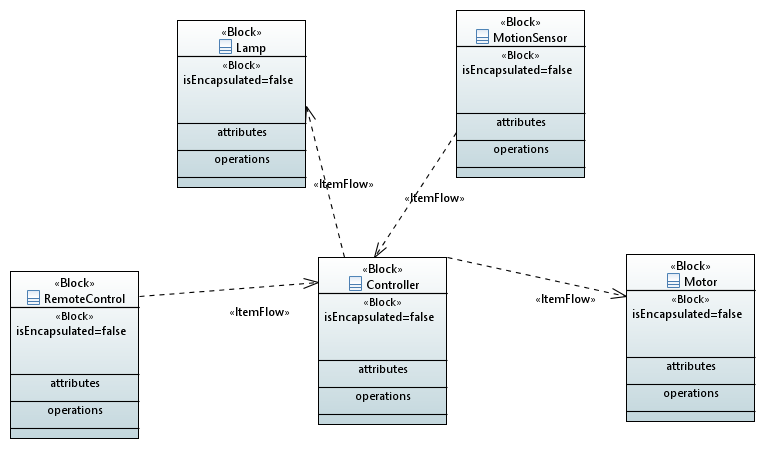
\includegraphics[width=100mm, keepaspectratio]{figures/BDDgarageSystem.png}
	\caption{Garage system physical components}
	\label{fig:GarageBDD}
\end{figure}

The \figref{GateControler} figure introduce the communication between the above listed blocks.

\begin{figure}[!ht]
	\centering
	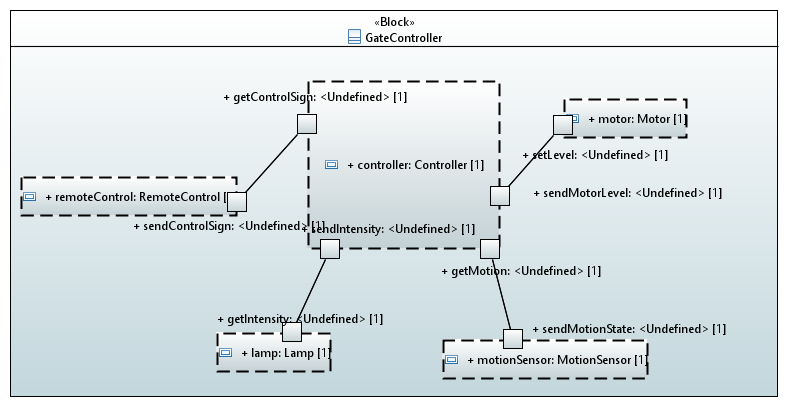
\includegraphics[width=150mm, keepaspectratio]{figures/IBDGateController.png}
	\caption{Gate controller internal block diagram}
	\label{fig:GateControler}
\end{figure}

A garage gate fundamentally have 2 main states, the \textit{Opened} and \textit{Closed} states, which is shown below on \figref{Garage Statemachine} figure, with orange colours.  First of all we can start from the \textit{Closed} state, where we can open the gate with an 'open' command. This command sets the state machine in an \textit{Opening} state. While opening the gate, somebody or something can move into the way, so this becomes \textit{Block Opening}. The gate is opening, if the blocking stops. After the \textit{Opening} phase succeeded the gate is \textit{Opened}. In this state we can 'close' the gate with a simple command, and the state machine goes to the \textit{Closing} state. There could be also a blocking action, which stops the closing movement. From this state the gate is starting the closing movement again after a few seconds \textit{Lighting}. When the closing action finished the gate is \textit{Closed}.

\begin{figure}[!ht]
\centering
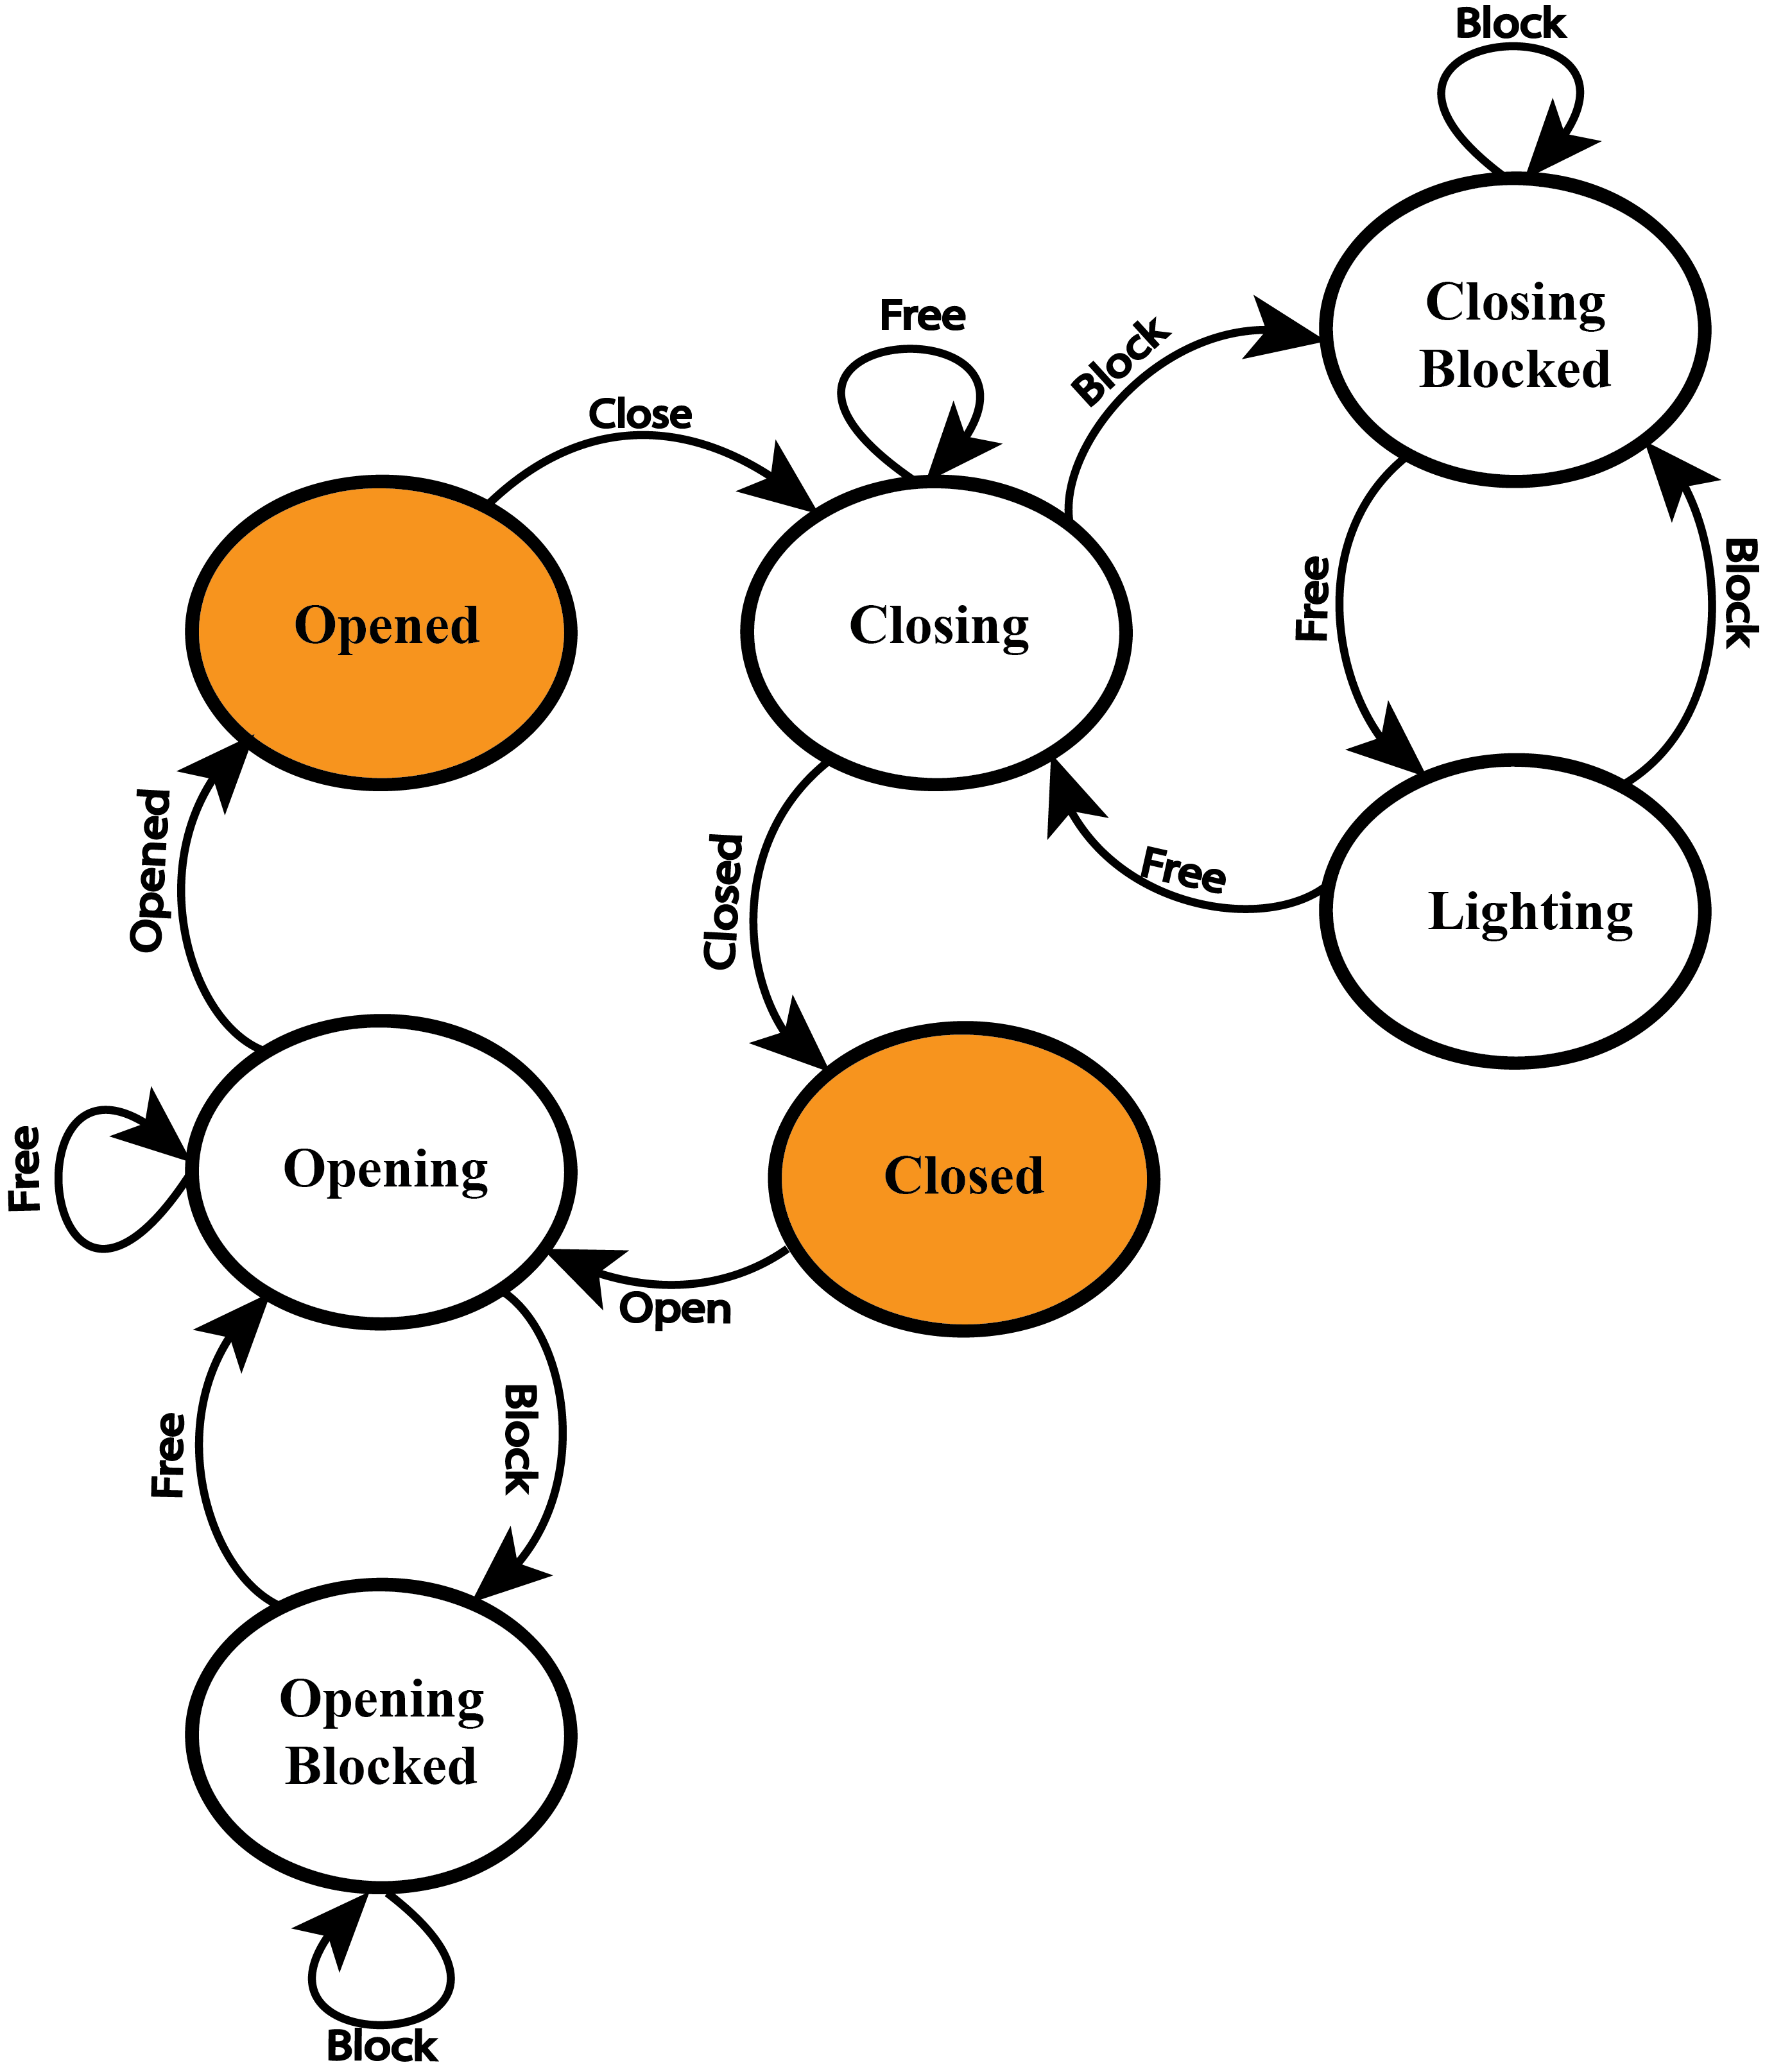
\includegraphics[width=100mm, keepaspectratio]{figures/garageState.png}
\caption{Garage gate state machine diagram}
\label{fig:Garage Statemachine}
\end{figure}

%TODO define what testing scenarios i will use
\paragraph{Testing goals}
The tests should achieve all the possible states of the SUT, because we want to detect the behaviour of the SUT in all use cases.